%% Copernicus Publications Manuscript Preparation Template for LaTeX Submissions
%% ---------------------------------
%% This template should be used for copernicus.cls
%% The class file and some style files are bundled in the Copernicus Latex Package, which can be downloaded from the different journal webpages.
%% For further assistance please contact Copernicus Publications at: production@copernicus.org
%% https://publications.copernicus.org/for_authors/manuscript_preparation.html





%% Please use the following documentclass and journal abbreviations for discussion papers and final revised papers.

%% 2-column papers and discussion papers
\documentclass[acp, manuscript]{copernicus}\usepackage[]{graphicx}\usepackage[]{color}
%% maxwidth is the original width if it is less than linewidth
%% otherwise use linewidth (to make sure the graphics do not exceed the margin)
\makeatletter
\def\maxwidth{ %
  \ifdim\Gin@nat@width>\linewidth
    \linewidth
  \else
    \Gin@nat@width
  \fi
}
\makeatother

\definecolor{fgcolor}{rgb}{0.345, 0.345, 0.345}
\newcommand{\hlnum}[1]{\textcolor[rgb]{0.686,0.059,0.569}{#1}}%
\newcommand{\hlstr}[1]{\textcolor[rgb]{0.192,0.494,0.8}{#1}}%
\newcommand{\hlcom}[1]{\textcolor[rgb]{0.678,0.584,0.686}{\textit{#1}}}%
\newcommand{\hlopt}[1]{\textcolor[rgb]{0,0,0}{#1}}%
\newcommand{\hlstd}[1]{\textcolor[rgb]{0.345,0.345,0.345}{#1}}%
\newcommand{\hlkwa}[1]{\textcolor[rgb]{0.161,0.373,0.58}{\textbf{#1}}}%
\newcommand{\hlkwb}[1]{\textcolor[rgb]{0.69,0.353,0.396}{#1}}%
\newcommand{\hlkwc}[1]{\textcolor[rgb]{0.333,0.667,0.333}{#1}}%
\newcommand{\hlkwd}[1]{\textcolor[rgb]{0.737,0.353,0.396}{\textbf{#1}}}%
\let\hlipl\hlkwb

\usepackage{framed}
\makeatletter
\newenvironment{kframe}{%
 \def\at@end@of@kframe{}%
 \ifinner\ifhmode%
  \def\at@end@of@kframe{\end{minipage}}%
  \begin{minipage}{\columnwidth}%
 \fi\fi%
 \def\FrameCommand##1{\hskip\@totalleftmargin \hskip-\fboxsep
 \colorbox{shadecolor}{##1}\hskip-\fboxsep
     % There is no \\@totalrightmargin, so:
     \hskip-\linewidth \hskip-\@totalleftmargin \hskip\columnwidth}%
 \MakeFramed {\advance\hsize-\width
   \@totalleftmargin\z@ \linewidth\hsize
   \@setminipage}}%
 {\par\unskip\endMakeFramed%
 \at@end@of@kframe}
\makeatother

\definecolor{shadecolor}{rgb}{.97, .97, .97}
\definecolor{messagecolor}{rgb}{0, 0, 0}
\definecolor{warningcolor}{rgb}{1, 0, 1}
\definecolor{errorcolor}{rgb}{1, 0, 0}
\newenvironment{knitrout}{}{} % an empty environment to be redefined in TeX

\usepackage{alltt}



%% Journal abbreviations (please use the same for discussion papers and final revised papers)


% Advances in Geosciences (adgeo)
% Advances in Radio Science (ars)
% Advances in Science and Research (asr)
% Advances in Statistical Climatology, Meteorology and Oceanography (ascmo)
% Annales Geophysicae (angeo)
% Archives Animal Breeding (aab)
% ASTRA Proceedings (ap)
% Atmospheric Chemistry and Physics (acp)
% Atmospheric Measurement Techniques (amt)
% Biogeosciences (bg)
% Climate of the Past (cp)
% DEUQUA Special Publications (deuquasp)
% Drinking Water Engineering and Science (dwes)
% Earth Surface Dynamics (esurf)
% Earth System Dynamics (esd)
% Earth System Science Data (essd)
% E&G Quaternary Science Journal (egqsj)
% Fossil Record (fr)
% Geographica Helvetica (gh)
% Geoscientific Instrumentation, Methods and Data Systems (gi)
% Geoscientific Model Development (gmd)
% History of Geo- and Space Sciences (hgss)
% Hydrology and Earth System Sciences (hess)
% Journal of Micropalaeontology (jm)
% Journal of Sensors and Sensor Systems (jsss)
% Mechanical Sciences (ms)
% Natural Hazards and Earth System Sciences (nhess)
% Nonlinear Processes in Geophysics (npg)
% Ocean Science (os)
% Primate Biology (pb)
% Proceedings of the International Association of Hydrological Sciences (piahs)
% Scientific Drilling (sd)
% SOIL (soil)
% Solid Earth (se)
% The Cryosphere (tc)
% Web Ecology (we)
% Wind Energy Science (wes)


%% \usepackage commands included in the copernicus.cls:
%\usepackage[german, english]{babel}
%\usepackage{tabularx}
%\usepackage{cancel}
%\usepackage{multirow}
%\usepackage{supertabular}
%\usepackage{algorithmic}
%\usepackage{algorithm}
%\usepackage{amsthm}
%\usepackage{float}
%\usepackage{subfig}
%\usepackage{rotating}

%\usepackage{mathptmx}
\usepackage{newtxmath}
\usepackage{upgreek}

\newcommand\nd{\ensuremath{N_d}}
\newcommand\cdnc{\nd}
\newcommand\lwp{\ensuremath{\mathcal L}}
\newcommand\fc{\ensuremath{f_c}}
\newcommand\cf{\fc}
\newcommand\re{\ensuremath{r_e}}
\newcommand\ql{\ensuremath{q_l}}
\newcommand\qi{\ensuremath{q_i}}

\newcommand\erf{\ensuremath{\text{ERF}}}
\newcommand\erfaci{\ensuremath{\text{ERF}_\text{aci}}}
\newcommand\erfari{\ensuremath{\text{ERF}_\text{ari}}}
\newcommand\rfaci{\ensuremath{\text{RF}_\text{aci}}}
\newcommand\rfari{\ensuremath{\text{RF}_\text{ari}}}

\newcommand\lon{\ensuremath{\lambda}}
\newcommand\lat{\ensuremath{\phi}}

%% \usepackage{helvet}
%% \usepackage{sansmath}
%% \usepackage{etoolbox}
%% \AtBeginEnvironment{tikzpicture}{
%%   \sansmath \sf
%% }
%% \AtEndEnvironment{tikzpicture}{
%%   \unsansmath 
%% }

\usepackage[textsize=11pt]{todonotes}
\usepackage{wasysym}
\newcommand{\commentjm}[1]{\todo[inline, color=red!50]{$j_\mu$: #1}}
\newcommand{\commentjq}[1]{\todo[inline, color=blue!50]{\textit{JQ}: #1}}
\newcommand{\commenteg}[1]{\todo[inline, color=green!50]{\textit{EG}: #1}}
\newcommand{\commentms}[1]{\todo[inline, color=yellow!50]{\textit{MS}: #1}}
\IfFileExists{upquote.sty}{\usepackage{upquote}}{}
\begin{document}

\title{Separating radiative forcing by aerosol--cloud interactions and rapid
  cloud adjustments in the ECHAM--HAMMOZ aerosol--climate model using the method
  of partial radiative perturbations}

\Author[1]{Johannes}{M\"ulmenst\"adt}
\Author[2]{Edward}{Gryspeerdt}
\Author[1]{Marc}{Salzmann}
\Author[3]{Po--Lun}{Ma}
\Author[1]{Sudhakar}{Dipu}
\Author[1]{Johannes}{Quaas}

\affil[1]{Universit\"at Leipzig, Leipzig, Germany}
\affil[2]{Space and Atmospheric Physics Group, Imperial College London, London, United Kingdom}
\affil[3]{Pacific Northwest National Laboratory, Richland, Washington, USA}

%% The [] brackets identify the author with the corresponding affiliation. 1, 2, 3, etc. should be inserted.



\runningtitle{$\text{RF}_\text{aci}$ and rapid cloud adjustments in ECHAM--HAMMOZ}

\runningauthor{M\"ulmenst\"adt et al.}

\correspondence{Johannes M\"ulmenst\"adt (\href{mailto:johannes.muelmenstaedt@uni-leipzig.de}{johannes.muelmenstaedt@uni-leipzig.de})}



\received{}
\pubdiscuss{} %% only important for two-stage journals
\revised{}
\accepted{}
\published{}

%% These dates will be inserted by Copernicus Publications during the typesetting process.


\firstpage{1}

\maketitle



\begin{abstract}
  Using the method of offline radiative transfer modelling within the partial
  radiative perturbations (PRP) approach, the effective radiative forcing
  by aerosol--cloud interactions (\erfaci) in the ECHAM--HAMMOZ aerosol climate
  model is decomposed into a radiative forcing by anthropogenic cloud droplet
  number change and adjustments of the liquid water path and cloud fraction.
  The simulated radiative forcing by anthropogenic cloud droplet
  number change and liquid water path adjustment are of
  approximately equal magnitude at $-0.52$~\unit{W~m^{-2}} and
  $-0.53$~\unit{W~m^{-2}}, respectively, while the cloud fraction adjustment is
  somewhat weaker at $-0.31$~\unit{W~m^{-2}} (constituting 38\%, 39\%, and 23\%
  of the total \erfaci, respectively); geographically, all three \erfaci{} components
  in the simulation peak over China, the subtropical eastern ocean boundaries,
  the northern Atlantic and Pacific oceans, Europe, and eastern North America (in
  order of prominence).  Spatial correlations indicate that the temporal-mean
  liquid water path adjustment is proportional to the temporal-mean radiative
  forcing, while the relationship between cloud fraction adjustment and
  radiative forcing is less direct.  While the estimate of warm-cloud \erfaci{} is
  relatively insensitive to the treatment of ice and mixed-phase cloud overlying
  warm cloud, there are indications that more restrictive treatments of ice in
  the column result in a low bias in the estimated magnitude of the liquid water
  path adjustment and a high bias in the estimated magnitude of the droplet
  number forcing.  Since the present work is the first PRP decomposition of the
  aerosol effective radiative forcing into radiative forcing and rapid cloud
  adjustments, idealized experiments are conducted to provide evidence that the
  PRP results are accurate.  The experiments show that using low-frequency
  (daily or monthly) time-averaged model output of the cloud property fields
  underestimates the ERF, but three-hourly mean output is sufficiently frequent.
\end{abstract}


\copyrightstatement{TEXT}

\introduction %% \introduction[modified heading if necessary]
Following \citet{Boucher2013}, it has become common to distinguish between
radiative forcing (RF) by aerosol--cloud interactions (ACI) and rapid adjustments
to this radiative forcing, with the sum of the forcing (\rfaci) and the rapid adjustments
denoted as the effective radiative forcing (\erfaci).  In liquid-water clouds,
\rfaci\ arises from the increased availability of cloud condensation nuclei
(CCN) in a polluted atmosphere leading to higher droplet number \nd\ and smaller
effective radius \re\ at constant cloud liquid water path \lwp\
\citep{Twomey1977}.  The atmosphere responds to the higher-\nd, lower-\re\
clouds by various processes occurring on short timescales, leading to
adjustments in other cloud properties, including \lwp\ and cloud vertical and
horizontal geometric extent.

Physically, the most important adjustment mechanisms are suppression of
precipitation formation \citep{Albrecht1989} and enhanced cloud-edge dry-air
entrainment and droplet evaporation in the smaller-droplet clouds
\citep{Ackerman04}.  The former mechanism, in isolation, would lead to an
increase in cloud condensate and cloud fraction, and thus a negative adjustment to the radiative
forcing; the latter, in isolation, would lead to a decrease in cloud condensate
and thus a positive adjustment to the radiative forcing.  Since no mechanism
occurs in isolation in a coupled system \citep{Stevens2009}, the question of
whether the net adjustment is positive or negative is both difficult and
unresolved
\citep[e.g.,][]{Muelmenstaedt2018,Gryspeerdt2019a}.

One method by which aerosol effective radiative forcing is estimated is to
calculate the difference in top-of-atmosphere (TOA) radiative fluxes in
general-circulation models (GCMs) between runs with fixed sea-surface
temperature and present-day or preindustrial aerosol concentrations or emissions
\citep[e.g.,][]{Lohmann2010,Forster2016}.  This requires a GCM that includes the
relevant aerosol--radiation and aerosol--cloud interaction mechanisms. By
representing the optical properties of aerosol in the radiative transfer, the
radiative forcing by aerosol--radiation interactions (\rfari) can be estimated;
by representing the \nd\ dependence on aerosol activation during cloud
formation, \rfaci\ can be estimated; and by representing precipitation
suppression and enhanced evaporation in smaller-\re\ clouds, the adjustments to
\rfaci\ can be estimated.  (We exclude ice and mixed-phase cloud processes,
which introduce further complications, from this discussion.) These processes
occur on scales far below the resolved scale, so their representation in the GCM
requires parameterization.  Thus, the model is only imperfectly (if at all)
aware of subgrid-scale variability in the process rates and feedbacks between
the processes; relies on imperfect base-state cloud properties
\citep[e.g.,][]{Penner2006}; and only considers effects that are amenable to
parameterization, meaning that precipitation suppression is included in many
models but enhanced evaporation is not
\citep[e.g.,][]{Salzmann2010,Michibata2016,Zhou2017}.  Based on these
considerations, a prevalent view is that, from the standpoint of achieving GCM
fidelity, ACI are more difficult than aerosol--radiation interactions, and ACI
adjustments are more difficult than the ACI forcing.  On top of this, the usual
concerns about parametric uncertainty apply, so that the overall uncertainty on
GCM estimates of \erfaci\ is large \citep{Boucher2013}.  Nevertheless, the
ability of GCMs to produce a global estimate will assure their star will
continue to shine brightly in the firmament of \erf\ estimation methods until
competing methods overcome their own significant drawbacks.

In general, one might argue that knowing the uncertainty on each term in a sum
is a good first step towards attacking the uncertainty on the total; certainly,
this is consistent with the GCM paradigm of building up the total forcing from
parameterizations for each of the contributing processes, even if it is less
applicable to ``top-down'' estimates from the historical evolution of the
climate system.  Thus, we write the effective radiative forcing by aerosol
as
\begin{equation}
  \label{eq:f}
  F = F_\text{ari} + F_{\nd} + F_\lwp + F_{\cf},
\end{equation}
where $F_\text{ari}$ is the \rfari, $F_{\nd}$ is the \rfaci\ due to the increase
in \nd, and $F_\lwp$ and $F_{\cf}$ are the \lwp\ and cloud fraction (\cf)
adjustments to the \rfari\ and \rfaci.  Other adjustments, e.g., due to rapid
changes in land surface temperatures or atmospheric temperature and humidity
profiles, have been estimated as small in a previous study \citep{Heyn2017}.
Each of these terms maps fairly well onto a parameterization in the GCM: \rfari\
is parameterized in the radiative transfer, $F_{\nd}$ is parameterized in a
droplet activation scheme, the ACI part of $F_\lwp$ is parameterized in the
precipitation microphysics \citep[and, if enhanced evaporation becomes tractable
in the future, that component will presumably be parameterized in the turbulence
scheme; e.g.,][]{Guo2011,Neubauer2014}, and $F_{\cf}$ is parameterized in the
cloud cover scheme (although in our model the response to the perturbation is
indirect, via relative humidity changes subsequent to precipitation rate
changes); the only component that emerges from the model dynamics rather than
from an explicit parameterization is the adjustments of temperature and moisture
profiles that entail further adjustments to aerosol--cloud interactions and to
aerosol--radiation interactions (formerly known as ``semi-direct effect''); both
of these terms are small \citep{Heyn2017,Stjern2017}.  A natural first step
would then be to ask how large each of these terms is, and a natural second step
would be to ask how much uncertainty each contributes to the total.  One of the
benefits of such a decomposition would be that it would provide a more solid
footing for---or falsify---the notion that models agree fairly well on the
``simpler'' problem of \rfaci\ and not well at all on the ``harder'' problem of
the adjustments.  However, performing the decomposition is quite difficult in
practice.  \citet{Ghan2013} addresses the issue of separating $F_\text{ari}$
from $F_{\nd} + F_\lwp + F_{\cf}$ using the model's intrinsic knowledge of the
anthropogenic perturbations.  It would be desirable to separate the three
\erfaci\ components analogously, using the intrinsic model knowledge of the time-varying, three-dimensional
aerosol perturbation and resulting perturbation of cloud properties.  However, 
methods that attempt to do so
need to
contend with the problem that \erfaci\ is diagnosed from two separate runs
that cannot easily share fields online, so that double radiation calls as in
\citet{Ghan2013} are not feasible; furthermore, even if double radiation calls
could be made, this would be of little help in estimating adjustments, which, by
definition, do not respond to the aerosol perturbations instantaneously.  One
method to estimate \erfaci\ components is the approximate partial radiative
perturbation (APRP) decomposition \citep{Taylor2007,Zelinka2014}.  APRP
decomposes the cloud property changes into changes in area fraction, cloud
albedo, and cloud absorption; the change in area fraction maps well onto the
\cf\ adjustment in the forcing--adjustment framework, but the APRP cloud albedo
change includes both the effect of the anthropogenic \nd\ change and the \lwp\
adjustment.  Another method is to deactivate the parameterized
precipitation suppression (and, if models include a parameterization of the
enhanced evaporation, deactivate that as well); however, the model with
parameterized adjustments will produce a different climate than the model
without \citep{Penner2006}.  Due to the complications arising in methods that
directly use the model state, less direct methods have been developed that
idealize the cloud field as a globally homogeneous single layer \citep{Ghan2016}
or use similar regression-based statistical techniques as satellite studies
\citep{Gryspeerdt2019b}.

In this work, we apply the method of partial radiative perturbations
\citep[PRP;][]{Wetherald1988,Colman1997,Colman2003,Klocke2013} to the ERF
decomposition problem.  PRP falls in the category of methods that
directly use the intrinsic model knowledge of the time-varying,
three-dimensional aerosol perturbation and resulting perturbation of cloud
properties.  The starting point for PRP is a
perturbed and an unperturbed model run.  One then introduces the fields of the
perturbed run into the unperturbed run, one at a time, and reruns the radiative
transfer scheme on the ``partially perturbed'' state to derive the resulting
change in radiative fluxes.  In our application, the two runs are
simulations with an atmospheric GCM with prescribed climatological,
seasonally varying sea surface temperature (SST) and sea ice cover (SIC) distributions
with present-day and preindustrial aerosol emissions, nudged to 
present-day large-scale upper-level winds to reduce the internal variability
without overconstraining the behavior of lower-tropospheric warm cloud and allow
significant changes in cloud property to emerge after a shorter integration time
than would otherwise be required \citep[e.g.,][]{Kooperman2012,Zhang2014}.  The perturbed fields are \nd, \lwp, and \cf;
the corresponding changes in radiative fluxes are $F_{\nd}$, $F_\lwp$, and
$F_{\cf}$.  

In Section~\ref{sec:method}, we describe the PRP method and
ECHAM--HAMMOZ model in detail; in
Section~\ref{sec:experiments}, we use PRP to estimate the ERF components in the
ECHAM--HAMMOZ model and determine whether the adjustments are a simple proportional
response to the forcing.  

\section{Methods}
\label{sec:method}

We first give a brief formal description of the PRP method; we then describe the
model configurations to which we will apply the method.

\subsection{Partial radiative perturbations}

We denote the shortwave TOA flux as $Q$ and the longwave flux as $R$ (all-sky,
positive downward in both cases).  For the purposes of this analysis, the radiative flux in
each spectral range is considered a function of the cloud properties \nd, \lwp\
(or the vertically resolved analogue \ql),
and \cf.  The dependence of the fluxes on other climate state variables -- water
vapor mixing ratio $q$; ice-water particle size, shape, and mixing ratio \qi;
aerosol properties; radiatively active gases; surface properties; and incoming
solar radiation -- is implicit:
\begin{align}
  \label{eq:fluxes}
  Q(\lon,\lat,t) &= Q(\nd(\lon,\lat, p,t), \ql(\lon,\lat,p,t), \cf(\lon,\lat,p,t)) \\
  R(\lon,\lat,t) &= R(\nd(\lon,\lat, p,t), \ql(\lon,\lat,p,t), \cf(\lon,\lat,p,t)) 
\end{align}

Let $\vec{x}^A = \{\nd^A, \lwp^A, \cf^A\}$ and
$\vec{x}^B = \{\nd^B, \lwp^B, \cf^B\}$ denote the cloud properties in runs $A$ and
$B$.  We then define \textit{forward} and \textit{backward} PRP as inserting one
cloud property at a time from one run into the cloud field of the other and
recalculating the radiative fluxes:
\begin{align}
  \label{eq:prp-fw-bk}
  \delta_{A\rightarrow B} Q_\xi & = Q(\{x_\xi^A, x_{\zeta{}\neq \xi}^B\}) - Q(\vec{x}^B) \\
  \delta_{B\rightarrow A} Q_\xi & = Q(\{x_\xi^B, x_{\zeta{}\neq \xi}^A\}) - Q(\vec{x}^A),
\end{align}
where $\delta$ denotes the difference in TOA flux when cloud
property $\xi$ is substituted from run $A$ into run $B$ or run $B$ into run 
$A$, respectively, and $Q$ (or $R$, analogously) is recalculated using the offline
version of the model's radiative transfer scheme.  \textit{Forward--backward} PRP is
simply the average of the two, taking into consideration that reversing
direction reverses the sign of the radiative-flux perturbation \citep[e.g.,][]{Klocke2013}:
\begin{equation}
  \label{eq:prp}
  \delta_{A\leftrightarrow B} Q_\xi = \frac{\delta_{A\rightarrow B} Q_\xi - \delta_{B\rightarrow A} Q_\xi} 2
\end{equation}

When $A$ denotes the preindustrial (PI)-emissions run and $B$ denotes the
present-day (PD)-emissions run, the
components of \erfaci\ correspond to
\begin{align}
  \label{eq:prp-fnd}
  F_{\nd}  &= \overline{\delta_{\text{PI}\leftrightarrow\text{PD}} Q_{\nd}  + \delta_{\text{PI}\leftrightarrow \text{PD}} R_{\nd}} \\
  \label{eq:prp-flwp}
  F_{\lwp} &= \overline{\delta_{\text{PI}\leftrightarrow \text{PD}} Q_{\lwp} + \delta_{\text{PI}\leftrightarrow \text{PD}} R_{\lwp}} \\
  \label{eq:prp-ffc}
  F_{\cf}  &= \overline{\delta_{\text{PI}\leftrightarrow \text{PD}} Q_{\cf}  + \delta_{\text{PI}\leftrightarrow \text{PD}} R_{\cf}}.
\end{align}
For other meanings of $A$ and $B$, as in the additional experiments performed in
Sections~\ref{sec:fsst}--\ref{sec:ice}, the equivalent expressions to
Equations~(\ref{eq:prp-fnd})--(\ref{eq:prp-ffc}) describe pseudo-forcing
components rather than forcing components; we denote them as $\tilde{F}_{\nd}$,
$\tilde{F}_{\lwp}$, and $\tilde{F}_{\cf}$.

In Equations~(\ref{eq:prp-fnd})--(\ref{eq:prp-ffc}),
\begin{equation}
  \label{eq:tempav}
  \overline{\mathcal{F}} = \frac 1 N \sum\limits_{i = 1}^N  \mathcal{F}(t_i)
\end{equation}
indicates averaging over the time dimension of a field $\mathcal{F}$ evaluated
at the $N$ time steps $\{t_1,\dots,t_N\}$.  ``Evaluated'' can, itself, refer to
a temporal average over the interval between evaluation time steps, as in a
3-hourly or daily mean, or it can refer to the instantaneous value of the field
at that time step; when the distinction matters (because $Q$ and $R$ are not
linear functions of their input variables), we will indicate the averaging
interval as $\overline{\mathcal{F}}{}^{(\Delta t)}$.  Thus,
$\overline{\mathcal{F}}{}^{(\text{inst})}$ denotes the temporal mean of
instantaneous model output, while $\overline{\mathcal{F}}{}^{(3~\text{h})}$
denotes the temporal mean of 3-hourly-averaged model output.


\subsection{Model description}

We use several model runs performed with the ECHAM--HAMMOZ model, version
echam6.1--ham2.2--moz0.9 \citep{Neubauer2014}.  The model is based on the ECHAM
atmospheric general circulation model \citep{Stevens2013}, the HAM interactive
aerosol module \citep{Stier2005,Zhang2012}, and the trace-gas chemistry module
MOZ \citep{Kinnison2007} (the latter is disabled in these runs).  Of most direct
relevance to our study, the parameterized processes contributing to
warm-cloud--aerosol interactions are aerosol activation into cloud droplets
according to \citet{Lin1997}; diagnostic warm rain processes (autoconversion and
accretion) according to \citet{Khairoutdinov2000}; and aerosol scavenging
according to \citet{Croft2009,Croft2010}.  The stratiform cloud scheme is that
of \citet{Lohmann1996}, extended to double-moment microphysics by
\citet{Lohmann2007} and \citet{Lohmann2009}, with the \citet{Sundqvist1989}
critical-relative-humidity cloud cover parameterization.

To reduce internal variability and achieve low statistical uncertainty on the
forcing components within a reasonable integration time, we use monthly
varying but yearly repeating SST and SIC from the observed
climatology and nudge the
large-scale wind fields to the present-day ERA-Interim reanalysis \citep{Dee2011} wind fields
of the years 2000--2010 (in some sensitivity studies, only the year 2000 is
used). 

Estimates of radiative forcing are computed by performing a pair of model runs
with present-day SST, SIC, and wind fields, and aerosol (precursor) emissions
estimates for either the year 2000 or the year 1850.  Emissions are from the
AEROCOM-II ACCMIP dataset; in particular, anthropogenic emissions follow
\citet{Lamarque2010}.  

To perform PRP on the model output, we have updated the offline version of the
RRTM-based ECHAM6 radiative transfer code \citep{Pincus2013} that was originally
used in \citet{Klocke2013}.   We use climatological aerosol mixing ratios 
\citep{Kinne2013} rather than the model's time-varying aerosol fields for aerosol--radiation
interactions; this reduces technical complexity as well as the volume of model
output needed to perform the PRP calculation.  To the extent that aerosol
overlying cloud is a small effect, this choice mainly affects our estimate of
the \cf\ adjustment \citep{Ghan2013,Zelinka2014}, which, unlike the \nd\ forcing
and \lwp\ adjustment, is straightforward to compute without the PRP machinery;
comparison to \citet{Gryspeerdt2019b} shows that the \cf\ adjustment estimate is
not strongly affected by this simplification.

When clouds are absent (or the cloud fraction is very low) in one run and
present in the other, perturbing cloud properties can yield unrealistically
large or small $q_l$ or $N_d$ (and thus $r_e$); this ``decorrelation'' problem
is well known from the application to climate feedbacks \citep{Colman1997} in
the context of the correlation between water vapor and cloudiness.  We allow the
radiative transfer code to resolve the conflicting cloud properties in the same
way as it does when the cloud microphysics and cloud cover schemes produce
conflicting cloud properties; in particular, $r_e$ can only vary within the
limits of the cloud optics lookup table used by the model ($2\times10^{-6}$ to
$32\times10^{-6}$~\unit{m}).  Appendices~\ref{sec:decorr} and \ref{sec:ideal}
describe tests we performed to verify that forward--backward PRP \erfaci\
estimates are not impacted by the decorrelation problem.

\section{Results}
\label{sec:experiments}

Since the components of the \erfaci\ have not been diagnosed before in
ECHAM--HAMMOZ by any method, we begin by presenting their global-mean values and
geographic distributions in Section~\ref{sec:fsst}.  In
Section~\ref{sec:proportion}, we investigate whether rapid adjustments to the
Twomey forcing are proportional to $F_{\nd}$ in terms of their spatial patterns.
Section~\ref{sec:ice} investigates the sensitivity of the PRP results to the
treatment of model columns containing ice and mixed-phase clouds. In
Section~\ref{sec:temporal}, we determine how much temporal averaging is permissible
before the PRP estimate becomes inaccurate.  Sections~\ref{sec:decorr} and
\ref{sec:ideal} discuss whether PRP diagnoses the \erfaci\ components correctly
in the presence of decorrelation effects (i.e., effects of introducing one cloud
property from one run into an uncorrelated cloud field in another run).

\subsection{What are the \erfaci\ components in ECHAM--HAMMOZ?}
\label{sec:fsst}

Using the PRP decomposition, Equations (\ref{eq:prp-fnd})--(\ref{eq:prp-ffc}),
we can diagnose the contributions to the \erfaci\ from PD and PI-emission
fixed-SST model runs.  This is shown in Figure~\ref{fig:echam-ham} and
Table~\ref{tab:echam-ham}.  The longwave effective forcing due to
warm-cloud--aerosol interactions is small, as could be expected.  No single
forcing or adjustment dominates the shortwave \erfaci; the global-mean forcing
$F_{\nd}$ and \lwp\ adjustment $F_{\lwp}$ are of comparable magnitude at
$-0.52$~\unit{W~m^{-2}} and $-0.53$~\unit{W~m^{-2}}.  The cloud-fraction
adjustment $F_{\fc}$ at $-0.31$~\unit{W~m^{-2}} is the smallest of the
components, consistent with CMIP5 models but not with other AeroCom models
\citep{Zelinka2014,Ghan2016,Gryspeerdt2019b}.  Our decomposition agrees with the
results of \citet{Gryspeerdt2019b} to within 0.1~\unit{W~m^{-2}} but disagrees
with \citet{Ghan2016} (who estimate $F_{\lwp}/F_{\nd}\approx 5$, in contrast to
our estimate of $\approx 1$), which both use a very similar configuration of the
same version of ECHAM--HAMMOZ.  Research to understand the differences between our
decomposition and others is underway.  All results in this section are based on
3-hourly mean output, $\overline{F}{}^{(3~\text{h})}$. This is a commonly used
model output configuration, albeit at the expensive end of the spectrum from the
standpoint of storage space requirements.  We will justify this choice in
Section~\ref{sec:temporal}.

The geographic patterns of all components exhibit similar features.  In the
northern hemisphere, fairly strong forcing prevails over both oceans and over
most of the continents, with the exception of desert regions, northern Asia, and
the Arctic; over the continents, a plume of high forcing components over China,
extending eastwards into the Pacific Ocean, and of a magnitude far greater than
over Europe and North America, is especially pronounced.  In the southern
hemisphere, on the other hand, sizable forcing components are largely limited to
the subtropical southern Pacific and southern Atlantic in the vicinity of the
persistent stratocumulus decks; smaller local maxima in the forcing components
also exist in the outflow regions of the midlatitude westerlies downwind of
South America, Africa, and Australia.

These geographic patterns result from a convolution of the distributions of
susceptible clouds and \nd\ perturbations.  Figure~\ref{fig:sens} shows the
\erfaci\ sensitivity, defined as the forcing or adjustment strength per
$e$-folding of the \nd\ burden (with the bar denoting temporal averaging
over the length of the run),
\begin{equation}
  \label{eq:sens}
  S_\xi = \frac{F_\xi}{\Delta \ln \overline{\mathcal{N}}_d}
\end{equation}
where the \nd\ burden is defined as
\begin{equation}
  \label{eq:burden}
  \mathcal{N}_d = \int N_d\,dz;
\end{equation}
Equation~(\ref{eq:sens}) is similar to the factorization of
\citet{Bellouin2020}.  The sensitivity for all \erfaci\ components is greater
over ocean than over land.  Over land, the most susceptible clouds can be found
over tropical Africa, southeastern Asia, and Central America; the anthropogenic
\nd\ perturbation over South America is too small to determine reliable
sensitivities.  Over ocean, the largest sensitivities occur in the midlatitudes,
near the equator, and over the eastern ocean boundaries; again, \nd\
perturbations in the southern hemisphere are too small to estimate sensitivities
reliably.  The regions of maximum sensitivity are the regions where the
base-state \lwp\ is high (not shown), which is intuitive in light of the strong
influence of \lwp\ on cloud albedo.

Figure~\ref{fig:deltand-filledcontour} shows the anthropogenic perturbation in
$\mathcal{N}_d$.  The perturbation is generally stronger over the continents
than over ocean; over ocean, it is generally strongest in the subtropics.  Thus,
the highest perturbations tend to coincide with the least susceptible clouds,
which explains why the \erfaci\ components exhibit far less variability over a
wide latitudinal range over the northern hemisphere oceans than either the
sensitivity or the \nd\ perturbation, and why the remote northern hemisphere
oceans are comparable to the polluted continental regions in \erfaci\ strength.
The exceptions to this pattern are the near-shore eastern ocean boundaries,
where a high sensitivity and reasonably strong \nd\ perturbation coincide,
and eastern China, where a reasonably high sensitivity and very strong \nd\
perturbation coincide.  The location where ECHAM--HAMMOZ simulates both the
strongest \nd\ forcing and the strongest \lwp\ adjustment is over land in China,
extending downwind into the northwestern Pacific Ocean.

In observational studies or observationally constrained modeling studies, it is
common to define susceptibilities analogously to Eq.~(\ref{eq:sens}) based on PD
variability in cloud and aerosol variables and then multiply those
susceptibilities by wholly or partially \citep{Bellouin2013,Kinne2019}
model-derived estimates of anthropogenic aerosol perturbations.  (In the
terminology we adopt here, ``sensitivity'' is a change in cloud property or
cloud radiative effect in response to a climatological change in an aerosol
variable, whereas ``susceptibility'' is a change in response to an instantaneous
change in an aerosol variable.)  Our results show that the most susceptible
oceanic clouds in this version of ECHAM--HAMMOZ occur where continental
pollution intrudes on relatively clean conditions over the eastern ocean
boundaries.  Some observational (or observationally constrained) studies agree
with this result \citep{Quaas2008,Alterskjaer2012,Engstrom2015,Gryspeerdt2016,
  Andersen2017, Christensen2017,McCoy2017}, while others disagree
\citep{Lebsock2008,Chen2014, Gryspeerdt2017}.  Of those studies that are not
restricted to oceanic clouds, some agree with our finding of strong forcing due
to relatively susceptible clouds over China \citep{Gryspeerdt2017,McCoy2017} and
some do not \citep{Quaas2008, Alterskjaer2012, Gryspeerdt2016}.

\subsection{Are the adjustments proportional to the forcing?}
\label{sec:proportion}

An intriguing aspect of the ACI problem is whether the adjustments may be
described approximately as a proportional response to the forcing
\citep{Gryspeerdt2019a}.  On the one hand, we do not necessarily expect
proportionality in the physical atmosphere, since the processes responsible for
the adjustments carry memory of the cloud evolution over various time scales;
the parameterized cloud processes in GCMs share this feature, at least in
principle, since the anthropogenic \cdnc\ perturbation seen by the precipitation
parameterization at one time step could be the result of a CCN perturbation at
some point in the past, carried to another point in space by advection, and
influenced by any of the other parameterized cloud processes.  On the other
hand, complex systems often exhibit simple emergent behaviors
\citep[e.g.,][and references therein]{Muelmenstaedt2018}.  If the adjustments
were to follow proportionally from the forcing, one consequence for the ACI
problem would be that the total \erfaci\ uncertainty should not be estimated as
the uncertainty on the sum of uncorrelated \rfaci\ and adjustments but rather
take the correlation between the forcing and adjustments into account, which
would result in a smaller \erfaci\ uncertainty estimate.  

In this study, we can test for proportionality in terms of the geographic
distribution using the spatial variability in
the temporal-mean \erfaci\ components.  Figure~\ref{fig:proportionality} shows that the zonal
mean of the ratio between \lwp\ adjustment and \nd\ forcing is relatively stable
around unity between the southern and northern midlatitudes with fairly small
interhemispheric differences except in the Southern Ocean.  The picture is
somewhat different for the ratio between \cf\ adjustment and \nd\ forcing, which
is more latitudinally variable and more different between the northern and
southern hemisphere.  Figure~\ref{fig:component-regression} reinforces these
conclusions, showing that $F_{\lwp}$ and $F_{\nd}$ are fairly tightly correlated
with a regression relationship remarkably close to one-to-one, while the
relationship between $F_{\cf}$ and $F_{\nd}$ is much looser.

One interpretation of these results is that the \erfaci\ components share a
geographic pattern due to the fact that large effects result from the
coincidence of large anthropogenic aerosol sources and susceptible clouds; the
shared geographic pattern then leads to an approximately proportional
relationship that breaks down farther from the source regions or where a
different mixture of cloud processes dominates the cloud response (e.g., the
Southern Ocean).  The cloud cover scheme, which diagnoses \cf\ from the grid
mean relative humidity, to some extent decouples \cf\ from the other cloud
properties, which attenuates the influence of \nd\ on \cf.  Nevertheless, the
vagueness of this argument is unsatisfactorily mismatched against the precision
of the $F_{\lwp}$--$F_{\nd}$ relationship, which suggests a deeper mechanism at
play, e.g., that precipitation acts as a common sink process for both \cdnc\ and
\lwp.

Further evidence for proportionality comes from \citep{Gryspeerdt2019b}, who
find an intermodel proportional relationship between global-mean forcing and
rapid adjustments.  

\subsection{How should we treat columns containing ice?}
\label{sec:ice}

In attempting to diagnose warm-cloud ACI forcing components, the question arises
how ice-containing clouds should be handled.  We can conduct the following set
of experiments to determine the range of forcing strengths associated with
different thermodynamic-phase treatments:
\begin{enumerate}
\item Perturb cloud properties in all cloudy model levels.\label{exp:all}
\item Perturb cloud properties in any liquid-containing cloudy model levels.\label{exp:mp}
\item Perturb cloud properties in liquid-only cloudy model levels (default).\label{exp:liq}
\item Perturb cloud properties in liquid-only cloudy columns.
\item Perturb cloud properties in liquid-only cloudy columns, correcting the
  result by their temporal occurrence fraction.
\end{enumerate}


Table~\ref{tab:phase} summarizes the results.  (For reasons of efficiency, we
performed these sensitivity experiments on daily-mean output, shortwave flux only.  We
did not perform experiment \ref{exp:mp} because we expect the result to lie
between experiments~\ref{exp:all} and \ref{exp:liq}, whose separation is already
in the noise.)  We conclude that how we choose to treat mixed-phase and ice
clouds makes little difference in ECHAM--HAMMOZ, so long as we do not restrict
ourselves to columns containing only warm clouds.  In the latter case,
correcting the forcing by the temporal occurrence fraction of liquid-only
columns in each model latitude--longitude box approximately recovers the results
when ice-containing columns are retained; however, there is some indication
of diverging trends in $F_{\nd}$ (which decreases in magnitude as the ice filtering becomes
more restrictive) and $F_{\lwp}$ (which increases in magnitude as the ice filtering becomes
more restrictive).  The ice-free column requirement is often made in
passive remote sensing studies to prevent contamination from ice clouds
overlying warm clouds and uncertainties in multilayer cloud retrievals.

\subsection{Does temporal averaging bias the results?}
\label{sec:temporal}

As Table~\ref{tab:temporal} shows, longer averaging periods underestimate the
forcing, but the differences between instantaneous output (the model time step
is 7.5~\unit{minutes}, but we sample every 3~\unit{h} to reduce the data volume)
and 3~\unit{h} averages is minimal.  Multimodel ensembles which archive
3~\unit{h} average output or 3~\unit{h} subsampled instantaneous of column cloud
properties, e.g., AeroCom and CFMIP2, are therefore amenable to treatment by the
PRP method.

\conclusions %% \conclusions[modified heading if necessary]
We have presented the first decomposition of the ACI effective forcing in
ECHAM--HAMMOZ into a Twomey forcing component and rapid adjustments of \lwp\ and
\fc.  In ECHAM--HAMMOZ, no single component dominates:
$F_{\nd} = -0.52$~\unit{W~m^{-2}}, $F_{\lwp} = -0.53$~\unit{W~m^{-2}}, and
$F_{\fc} = -0.31$~\unit{W~m^{-2}}; the Twomey forcing and \lwp\ adjustment are
approximately equally strong, and the \cf\ adjustment is somewhat weaker, as in
many other models.  The global ERF is dominated by the northern-hemisphere
forcing.  Within the northern hemisphere, the strongest forcing components occur
over land in China in $F_{\nd}$ and $F_{\lwp}$.  As expected, the stratocumulus
sheets over the eastern ocean basins also show strong responses in both
hemispheres, as do the midlatitude North Atlantic and North Pacific.

The temporal-mean spatial patterns of $F_{\nd}$ and $F_{\lwp}$ are highly
correlated, suggesting an effective proportionality in the \lwp\ adjustment to
the Twomey forcing even though the precipitation-suppression mechanism by which
the \lwp\ adjustment is parameterized in the model has inherent memory that
could decouple it from the Twomey effect.  The spatial patterns
of the temporal-mean $F_{\nd}$ and $F_{\lwp}$, while sharing some of the same
gross features, have a much less tight relationship than $F_{\nd}$ and
$F_{\lwp}$.

In our study of ECHAM--HAMMOZ, the forcing components are fairly insensitive to
how we treat columns containing both ice and liquid cloud condensate.  Requiring
that columns be free of ice and then correcting for the temporal fractional
occurrence of ice cloud, a technique that is often necessary in observational
studies, largely reproduces the results we obtain when we do not filter out such
columns, albeit possibly causing an overestimate of the \lwp\ adjustment and an
underestimate of the \nd\ forcing.  (In interpreting the bearing of these
results on analyses of satellite cloud retrievals, note that these studies do
not necessarily apply the ice-free requirement at the coarse GCM scales of the
present work, depending on whether they use gridded ``level 3'' data or the
``level 2'' native resolution of the retrieval algorithms.)

Through idealized sensitivity studies presented in the Appendix, we have showed
that PRP is a viable method for accurately decomposing \erfaci\ into a \nd\
forcing and \lwp\ and \cf\ adjustments.  This is the case despite large
artifacts that occur due to the decorrelated cloud property fields; the
forward--backward technique advocated by \citet{Colman1997} is capable of
removing these artifacts.

PRP directly uses the intrinsic model knowledge of the time-varying,
three-dimensional aerosol perturbation and resulting perturbation of cloud
properties to diagnose the \erfaci\ components and their
spatial patterns.  This makes it a useful tool for providing
context to other less resource-intensive decomposition methods \citep[e.g.,][]{Ghan2016,
  Gryspeerdt2019b} or to intercomparison studies \citep[e.g.,][]{Pincus2016,
  Smith2018} despite its demand for high-frequency vertically resolved model
output.

\appendix

\section{Validation of the PRP method for ACI decomposition}

\subsection{What is the effect of decorrelating the cloud properties?}
\label{sec:decorr}

Consider the results of forward and backward PRP plotted separately for the
PD--PI experiment in Figure~\ref{fig:fw-bk-pd-pi}.  Not only are the magnitudes
grotesque, but taken at face value, they would imply a positive forcing in one
direction and a negative forcing in the other.  Furthermore, the spatial
patterns bear no resemblance to that expected for \erfaci.  In this section, we
investigate the consequences of these features for the \erfaci\ decomposition.

Any given atmospheric property is often correlated with many others.
Substituting cloud properties one at a time breaks these correlations.  For
example, since ECHAM--HAMMOZ parameterizes precipitation suppression by aerosol, we
expect a positive correlation between \nd\ and \lwp\ within a model run.  If we
substitute \lwp\ from another run, the mechanistic link between \nd\ and \lwp\
through precipitation suppression, by which higher \nd\ at a given point in time
leads to higher \lwp\ at later times, is broken, and, therefore, the correlation
between \nd\ and \lwp\ is altered.

We estimate the strength of such decorrelation effects by performing two model
runs with (almost exactly) the same model physics, both nudged to the same
large-scale dynamics and with the same fixed SST; the only difference between
the runs is that a parameter in the \citet{Khairoutdinov2000} formulation for
the autoconversion rate, tuned for ECHAM--HAMMOZ,
\begin{equation}
  \label{eq:kk2000}
  Q_\text{aut} = \gamma q_l^\alpha \left(\frac{\nd}{1~\unit{cm^{-3}}}\right)^{-\beta},
\end{equation}
has been slightly perturbed from $\beta = 1.79$ to $\beta' = 1.79 + 10^{-5}$
($\alpha = 2.47$ and $\gamma = 4\times 1350~\unit{s^{-1}}$ are unchanged).  Even
over short integration times (a year), these model runs will converge on the
same climate, with nearly identical forcing components.  (The small perturbation
in $\beta$ does not result in a significant change in model sensitivity.)
However, at any given elapsed integration time and geographic location, the
cloud properties in the two runs are essentially uncorrelated.  We refer to this
pair of runs as the \textit{same-climate--different-weather experiment}.
Knowing that the true climatological TOA flux difference between this pair of
runs is zero, we can use these runs to estimate decorrelation effects between
any other decorrelated pair of runs, including the PD and PI emissions runs.

We find that decorrelation effects cause the PRP method to estimate enormous TOA
flux perturbations when we perform forward or backward substitution of any
single cloud property; this is shown in panels (a) and (b) of
Figure~\ref{fig:fw-bk}.  

Unlike forward PRP or backward PRP individually, forward--backward PRP is
unaffected by decorrelation, both in the global mean and locally in the temporal
mean: panel (c) of Figure~\ref{fig:fw-bk} shows that the fluctuations in
$\Delta Q$ rapidly (i.e., within a year) average to zero.  This confirms
that the \citet{Colman1997} prescription is successful at minimizing the
spurious effects of decorrelation.

\subsection{Does PRP give the right answer?}
\label{sec:ideal}

The preceding section provides evidence that strong decorrelation effects do not
lead to a spurious offset in forward--backward PRP results.  Next, we show that
decorrelation effects also do not lead to spurious scale factors.  To do so, we
scale \nd\ and \lwp\ by a globally constant factor of 1.1 at all timesteps and
scale \cf\ by 0.99. We use PRP to diagnose the forcing associated with each of
these perturbations; the results are shown in the first three rows of
Table~\ref{tab:ideal}.  We can then estimate the strength of the decorrelation
effects by performing PRP on the $\beta' = 1.79 + 10^{-5}$ run and the
scaled-$\{\nd,\lwp,\cf\}$ $\beta = 1.79$ run.  This is shown in the middle three
rows of Table~\ref{tab:ideal}; the correct results are recovered to good
approximation, with generally small attribution to incorrect \erfaci\ components
(the largest is $-0.05$~\unit{W~m^{-2}} incorrectly diagnosed as \fc\ adjustment
in the $\lwp\times 1.1$ experiment) and generally small differences between the
actual and diagnosed (the largest is a diagnosed
$F_{\lwp} = -0.48$~\unit{W~m^{-2}} when the correct value is
$-0.53$~\unit{W~m^{-2}}).  The final test is an experiment in which all cloud
properties are perturbed simultaneously and the clouds are decorrelated by using
a $\beta' = 1.79 + 10^{-5}$ baseline run.  The results are shown on the last
line of Table~\ref{tab:ideal}; the correct \erfaci\ components are recovered in
the presence of the confounding effects of decorrelation and of perturbing
multiple cloud properties simultaneously with $0.1$~\unit{W~m^{-2}} or better
accuracy, the largest discrepancy being the diagnosed
$F_{\cf} = 0.14$~\unit{W~m^{-2}} when the correct value is
$0.24$~\unit{W~m^{-2}}).

Thus, we find that forward--backward PRP can diagnose the forcing components
correctly in the presence of decorrelations, in addition to diagnosing the
absence of forcing correctly in the same-climate--different-weather case.

\subsection{Are the results sensitive to choosing grid-mean or in-cloud perturbations?}
\label{sec:in-cloud}

Perturbing in-cloud or grid-mean \cdnc\ and \lwp\ would be equivalent in the
limit in which TOA flux perturbations are linear in the cloud properties.  While
individual model columns do not satisfy this linearity requirement, the temporal
mean apparently exhibits sufficient effective linearity that the choice of
in-cloud or grid-mean perturbations has little effect on the ERF component
estimate; compare Tables~\ref{tab:echam-ham} and \ref{tab:in-cloud}.

\noappendix

%% \noappendix       %% use this to mark the end of the appendix section

%% %% Regarding figures and tables in appendices, the following two options are possible depending on your general handling of figures and tables in the manuscript environment:

%% %% Option 1: If you sorted all figures and tables into the sections of the text, please also sort the appendix figures and appendix tables into the respective appendix sections.
%% %% They will be correctly named automatically.

%% %% Option 2: If you put all figures after the reference list, please insert appendix tables and figures after the normal tables and figures.
%% %% To rename them correctly to A1, A2, etc., please add the following commands in front of them:

%% \appendixfigures  %% needs to be added in front of appendix figures

%% \appendixtables   %% needs to be added in front of appendix tables

%% %% Please add \clearpage between each table and/or figure. Further guidelines on figures and tables can be found below.

%% The following commands are for the statements about the availability of data sets and/or software code corresponding to the manuscript.
%% It is strongly recommended to make use of these sections in case data sets and/or software code have been part of your research the article is based on.

\codedataavailability{The PRP code is available in the GitHub repository
  jmuelmen/acp-2018-1304-echam-prp, archived under source-code DOI
  \url{https://doi.org/10.5281/zenodo.3457389}.  The analysis code is available
  in the GitHub repository jmuelmen/acp-2018-1304.  ECHAM--HAMMOZ is available
  from \url{https://hammoz.ethz.ch} subject to acknowledgment of a licensing
  agreement.  Due to the large data volume of 3-hourly vertically resolved
  fields, the model output itself was not archived, but model configuration
  files that can be used to replicate the output are available as part of the
  PRP code.  The PRP output on which the manuscript is based is available from
  the data DOI \url{https://doi.org/10.5281/zenodo.3457397}.}

\authorcontribution{$j_\mu$ designed the study, performed model runs, computed
  the PRP diagnostics, and drafted the manuscript.  EG and $j_\mu$ validated and
  debugged the results.  EG, MS, PM, JQ, and $j_\mu$ proposed various
  sensitivity studies.  EG, MS, PM, SD, JQ, and $j_\mu$ worked on the
  interpretation of the results.  All authors contributed text to or comments on
  the manuscript.}

\competinginterests{The authors declare that they have no competing interests.} %% this section is mandatory even if you declare that no competing interests are present

\begin{acknowledgements}
  We thank Christina Sackmann, Steve Ghan, and an anonymous reviewer for their
  insightful comments that have improved the manuscript.  The ECHAM--HAMMOZ
  model is developed by a consortium composed of ETH Zurich, Max-Planck-Institut
  für Meteorologie, Forschungszentrum Jülich, University of Oxford, and the
  Finnish Meteorological Institute and managed by the Center for Climate Systems
  Modeling (C2SM) at ETH Zurich.  This work was funded by the FLASH project
  (project number QU 311/14-1) in the HALO Priority Program (SPP 1294) of the
  German Research Foundation (Deutsche Forschungsgemeinschaft, DFG); by the
  European Union through European Research Council (ERC) Starting Grant QUAERERE
  (grant agreement 306284); by the German Federal Ministry of Education and
  Research within the Research for Sustainable Development (FONA) framework
  program under the \unit{HD(CP)^2} project (project number 01LK1504C).  EG was
  supported by an Imperial College London Junior Research Fellowship.  PM's
  contributions were supported by a travel grant from the Leibniz Invitations
  program at Universität Leipzig.  Computing resources were provided by the
  German Climate Computing Center (Deutsches Klimarechenzentrum, DKRZ).
\end{acknowledgements}




%% REFERENCES

%% The reference list is compiled as follows:

%% \begin{thebibliography}{}

%% \bibitem[AUTHOR(YEAR)]{LABEL1}
%% REFERENCE 1

%% \bibitem[AUTHOR(YEAR)]{LABEL2}
%% REFERENCE 2

%% \end{thebibliography}

%% Since the Copernicus LaTeX package includes the BibTeX style file copernicus.bst,
%% authors experienced with BibTeX only have to include the following two lines:
%%

\bibliographystyle{copernicus}
\bibliography{erf-clean.bib}
%%
%% URLs and DOIs can be entered in your BibTeX file as:
%%
%% URL = {http://www.xyz.org/~jones/idx_g.htm}
%% DOI = {10.5194/xyz}


%% LITERATURE CITATIONS
%%
%% command                        & example result
%% \citet{jones90}|               & Jones et al. (1990)
%% \citep{jones90}|               & (Jones et al., 1990)
%% \citep{jones90,jones93}|       & (Jones et al., 1990, 1993)
%% \citep[p.~32]{jones90}|        & (Jones et al., 1990, p.~32)
%% \citep[e.g.,][]{jones90}|      & (e.g., Jones et al., 1990)
%% \citep[e.g.,][p.~32]{jones90}| & (e.g., Jones et al., 1990, p.~32)
%% \citeauthor{jones90}|          & Jones et al.
%% \citeyear{jones90}|            & 1990



%% FIGURES

%% When figures and tables are placed at the end of the MS (article in one-column style), please add 
\clearpage
%% between bibliography and first table and/or figure as well as between each table and/or figure.


%% ONE-COLUMN FIGURES

%%f
%\begin{figure}[t]
%\includegraphics[width=8.3cm]{FILE NAME}
%% %% (/ 8.3 2.54)
%\caption{TEXT}
%\end{figure}
%
%%% TWO-COLUMN FIGURES
%
%%f
\begin{figure*}[t]
  \centering



{\centering 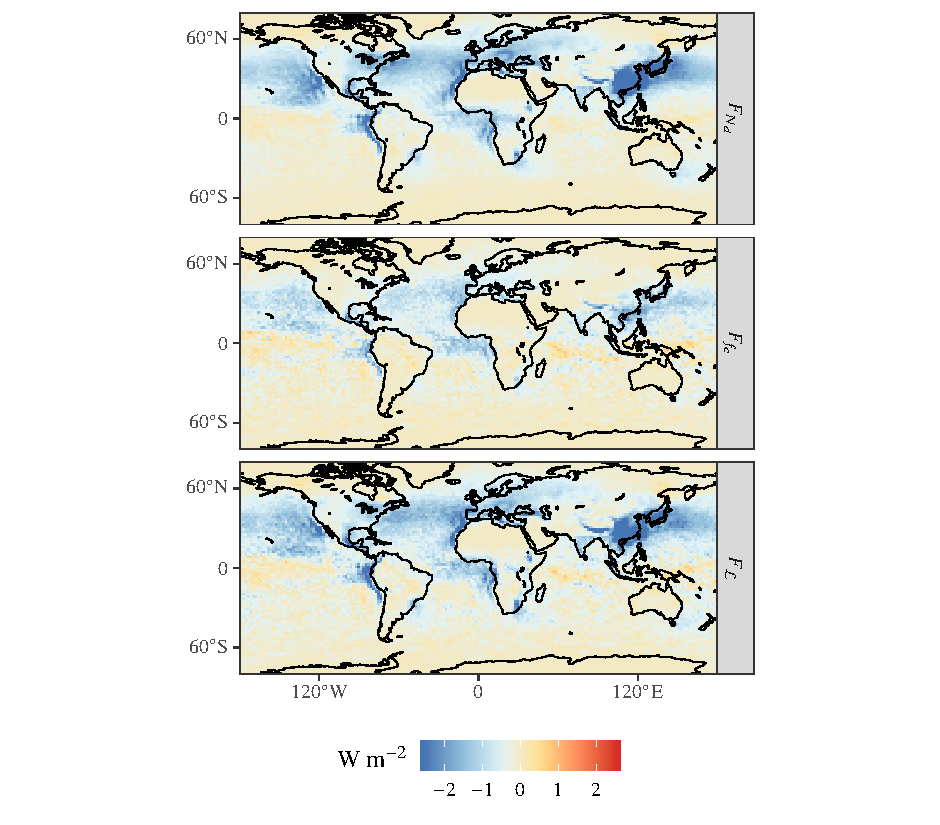
\includegraphics[width=\textwidth]{figure/erf-prp-erf-1} 

}



\caption{\erfaci\ components in ECHAM--HAMMOZ estimated by forward--backward PRP}
\label{fig:echam-ham}
\end{figure*}

\clearpage

\begin{figure*}[t]
  \centering



{\centering 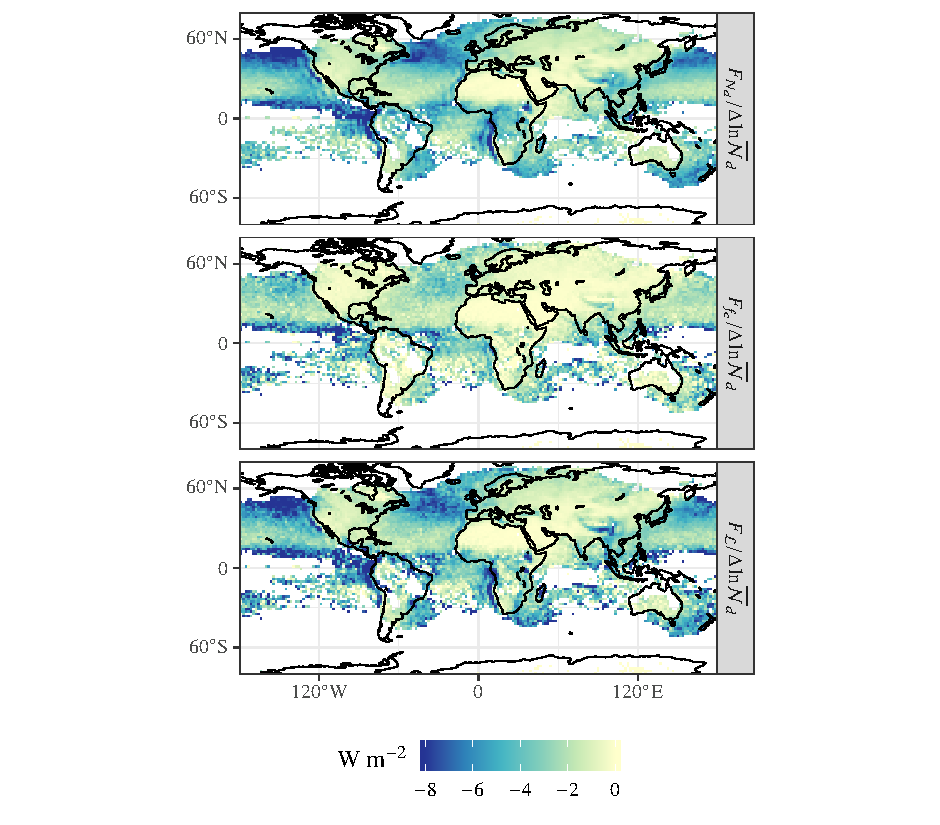
\includegraphics[width=\textwidth]{figure/erf-prp-erf-susc-1} 

}



  \caption{Sensitivity of \erfaci\ components to anthropogenic $\mathcal{N}_d$
    change (shown only where $\Delta\ln\overline{\mathcal{N}}_d > 0.05$)}
  \label{fig:sens}
\end{figure*}

\clearpage

\begin{figure}[t]
  \centering



{\centering 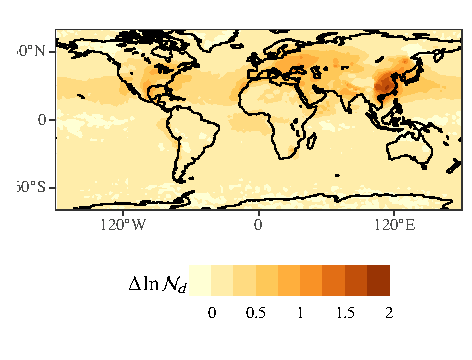
\includegraphics[width=0.5\linewidth]{figure/erf-prp-delta-ln-nd-filled-contour-1} 

}



  \caption{Anthropogenic $\ln\mathcal{N}_d$ change}
  \label{fig:deltand-filledcontour}
\end{figure}

\clearpage

\begin{figure}[t]
  \centering



{\centering 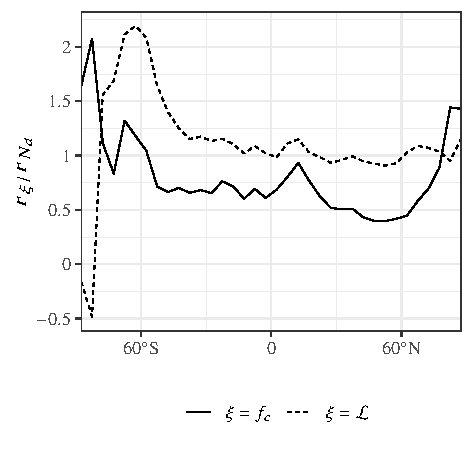
\includegraphics[width=8cm]{figure/erf-prp-erf-ratios-1} 

}



  
  \caption{\erfaci\ adjustments relative to the Twomey forcing}
\label{fig:proportionality}
\end{figure}

\clearpage

\begin{figure*}[t]
  \centering



{\centering 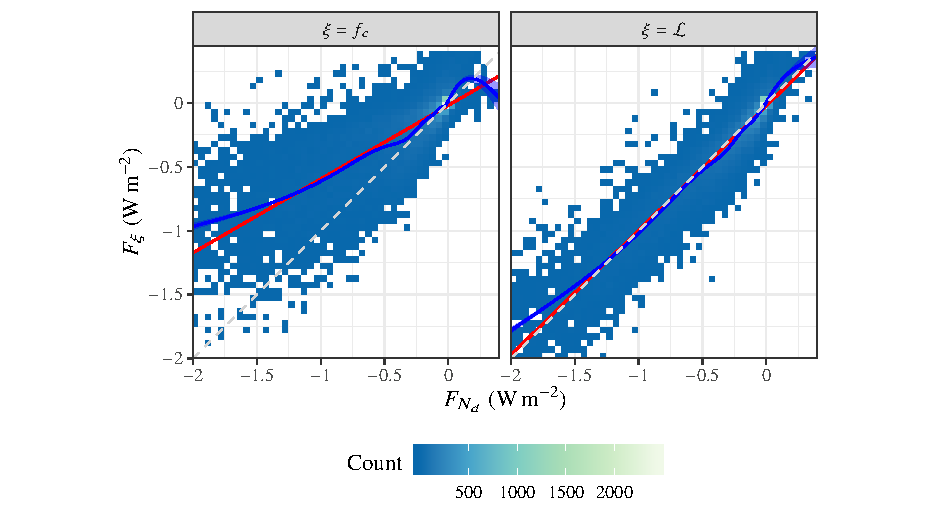
\includegraphics[width=\textwidth]{figure/erf-prp-erf-regress-1} 

}




%% %% (/ 12 2.54)

\caption{Correlation plots between the temporal-mean Twomey forcing and the adjustments; color
  indicates the number of grid boxes within each
  $0.05~\unit{W~m^{-2}} \times 0.05~\unit{W~m^{-2}}$ bin; the red line is a
  linear least-squares regression; the blue line is a generalized additive model
  regression \citep{Wood2011}, with 95\% confidence interval shaded in light
  blue; and the dashed gray line is the one-to-one line}
\label{fig:component-regression}
\end{figure*}

\clearpage

\appendixfigures

\begin{figure*}[t]
  \centering
  


{\centering 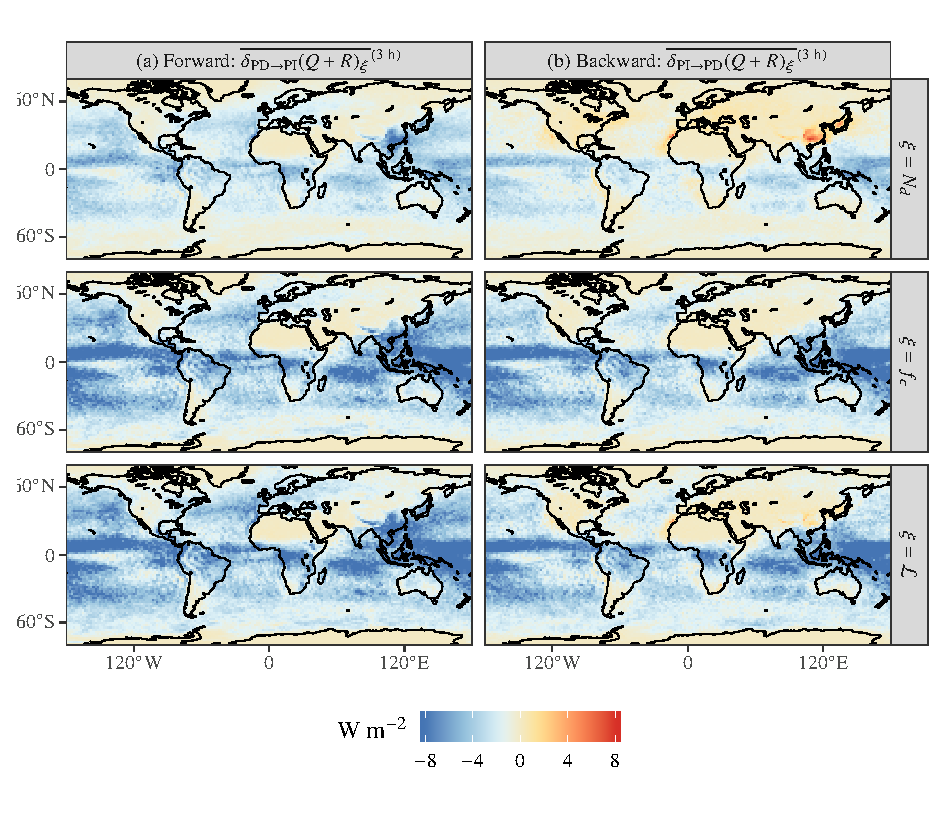
\includegraphics[width=\textwidth]{figure/erf-prp-erf-fw-pd-pi-1} 

}



\caption{Forward (a) and backward (b) PRP estimates of the \erfaci\ components.
  Note the significantly wider color scale than in Figure~\ref{fig:echam-ham}.}
  \label{fig:fw-bk-pd-pi}
\end{figure*}

\clearpage

\begin{figure*}[t]
  \centering
  


{\centering 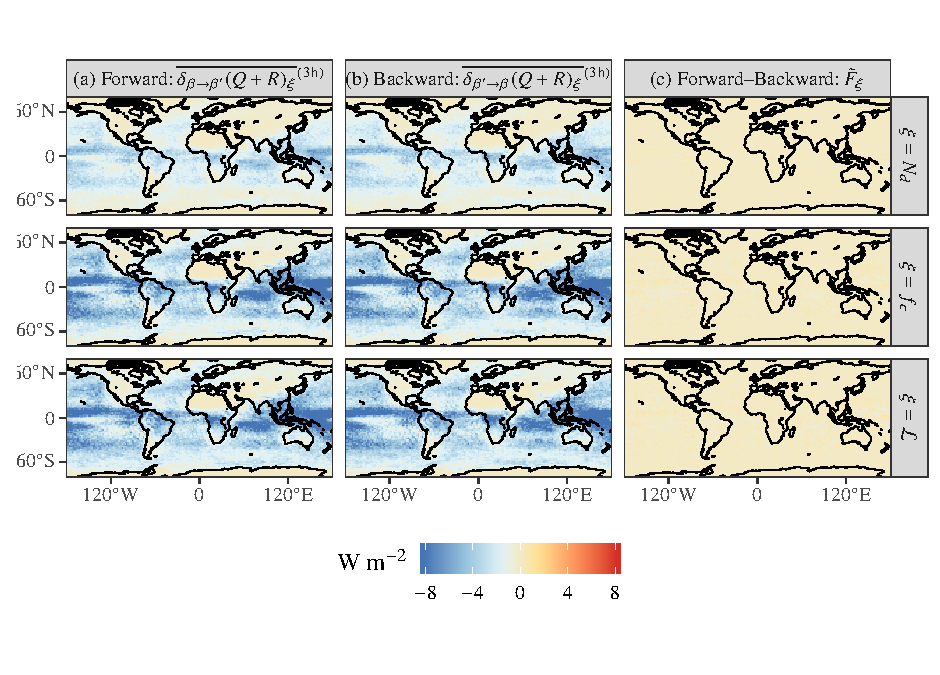
\includegraphics[width=\textwidth]{figure/erf-prp-erf-fw-1} 

}



  \caption{Forward (a), backward (b), and (c) forward--backward PRP performed on the
    same-climate--different-weather case.  Note the significantly wider color scale than in Figure~\ref{fig:echam-ham}.}
  \label{fig:fw-bk}
\end{figure*}

%% \appendixfigures

% 
%
%%% TABLES
%%%
%%% The different columns must be seperated with a & command and should
%%% end with \\ to identify the column brake.
%
%%% ONE-COLUMN TABLE
%
%%t
%\begin{table}[t]
%\caption{TEXT}
%\begin{tabular}{column = lcr}
%\tophline
%
%\middlehline
%
%\bottomhline
%\end{tabular}
%\belowtable{} % Table Footnotes
%\end{table}
%

\clearpage

\begin{table*}[t]
  \caption{\erfaci\ components in ECHAM--HAMMOZ estimated by forward--backward PRP.
    The total ERF also includes the ice-phase ACI effects ($-0.59$~W~m$^{-2}$ in
    the SW, $0.88$~W~m$^{-2}$ in the LW), \rfari{} ($-0.17$~W~m$^{-2}$ in the SW),
    and a negligible surface-albedo contribution ($-0.01$~W~m$^{-2}$), estimated
    for a very similar model run in \citet{Gryspeerdt2019b}.  The sum of the
    components thus balances at approximately the 0.2~W~m$^{-2}$ level, a
    relative error similar to the 0.1~W~m$^{-2}$ estimated uncertainty on the
    \erfaci{} components.}
  \label{tab:echam-ham}
  \centering
  \begin{tabular}{c|rrr|r|r}
  \hline\hline
    & \multicolumn{3}{c|}{ERF components (W m$^{-2}$)}
    & \multicolumn{1}{c|}{Sum (W m$^{-2}$)} 
    & \multicolumn{1}{c}{Total ERF (W m$^{-2}$)} \\


% latex table generated in R 3.4.4 by xtable 1.8-2 package
% Mon Feb 11 15:43:06 2019
Spectrum & $F_{\cdnc}$ & $F_{\cf}$ & $F_{\lwp}$ & \multicolumn{1}{c|}{$F_{\cdnc} + F_{\cf} + F_{\lwp}$} &   \\ 
  \hline
LW & 0.00 & 0.04 & 0.03 & 0.07 & 0.72 \\ 
  SW & $-$0.52 & $-$0.35 & $-$0.57 & $-$1.44 & $-$2.03 \\ 
   \hline
\hline

  \end{tabular}
\end{table*}

\clearpage

\begin{table*}[t]
  \caption{Dependence of diagnosed \erfaci\ components on treatment of
    thermodynamic phase}
  \label{tab:phase}
  \centering
  \begin{tabular}{l|rrr}
  \hline\hline
    & \multicolumn{3}{c}{ERF components (W m$^{-2}$)}\\
% latex table generated in R 3.4.4 by xtable 1.8-2 package
% Mon Feb 11 15:43:07 2019
Phase treatment & $\delta Q_{\cdnc}$ & $\delta Q_{\cf}$ & $\delta Q_{\lwp}$ \\ 
  \hline
All phases & $-$0.29 & $-$0.29 & $-$0.34 \\ 
  Liquid-only cloudy model levels & $-$0.27 & $-$0.27 & $-$0.35 \\ 
  Liquid-only cloudy model columns & $-$0.15 & $-$0.17 & $-$0.21 \\ 
  Liquid-only cloudy model columns (corrected for occurrence fraction) & $-$0.26 & $-$0.29 & $-$0.38 \\ 
   \hline
\hline

  \end{tabular}
\end{table*}



\clearpage

\begin{table}[t]
  \caption{Dependence of diagnosed \erfaci\ components on temporal averaging}
  \label{tab:temporal}
  \centering
  \begin{tabular}{c|rrr}
  \hline\hline
    & \multicolumn{3}{c}{ERF components (W m$^{-2}$)}\\
% latex table generated in R 3.4.4 by xtable 1.8-2 package
% Mon Feb 11 15:43:07 2019
Averaging period & $F_{\cdnc}$ & $F_{\cf}$ & $F_{\lwp}$ \\ 
  \hline
1~\unit{month} & $-$0.09 & $-$0.09 & $-$0.11 \\ 
  1~\unit{d} & $-$0.35 & $-$0.33 & $-$0.30 \\ 
  3~\unit{h} & $-$0.52 & $-$0.31 & $-$0.53 \\ 
  instantaneous & $-$0.55 & $-$0.30 & $-$0.51 \\ 
   \hline
\hline

  \end{tabular}
\end{table}

\clearpage

\appendixtables

\begin{table*}[t]
  \caption{\erfaci\ components resulting from idealized perturbations to \nd,
 \lwp, and \cf; estimate of the same \erfaci\ components by
    forward--backward PRP in the presence of decorrelation effects.}
  \label{tab:ideal}
  \centering
  \begin{tabular}{c|rrr}
  \hline\hline
    & \multicolumn{3}{c}{ERF components (W m$^{-2}$)}\\
% latex table generated in R 3.4.4 by xtable 1.8-2 package
% Mon Jun 10 15:24:47 2019
Perturbation & $F_{\cdnc}$ & $F_{\cf}$ & $F_{\lwp}$ \\ 
  \hline
$\nd\times 1.1$ & $-$0.38 & $-$0.00 & $-$0.00 \\ 
  $\cf\times 0.99$ & $-$0.00 & 0.24 & $-$0.00 \\ 
  $\lwp\times 1.1$ & $-$0.00 & $-$0.00 & $-$0.53 \\ 
   \hline
$\nd\times 1.1$ with $\beta' = \beta + 10^{-5}$ & $-$0.37 & $-$0.01 & $-$0.01 \\ 
  $\cf\times 0.99$ with $\beta' = \beta + 10^{-5}$ & 0.01 & 0.21 & 0.02 \\ 
  $\lwp\times 1.1$ with $\beta' = \beta + 10^{-5}$ & 0.01 & $-$0.05 & $-$0.48 \\ 
   \hline
$\nd\times 1.1, \lwp\times 1.1, \cf\times 0.99$ with $\beta' = \beta + 10^{-5}$ & $-$0.31 & 0.14 & $-$0.49 \\ 
   \hline
\hline

  \end{tabular}
\end{table*}

\clearpage

\begin{table}[t]
  \caption{\erfaci\ components calculated by PRP on \fc\ and in-cloud \nd\ and
    \ql}
  \label{tab:in-cloud}
  \centering
  \begin{tabular}{rrr}
  \hline\hline
    \multicolumn{3}{c}{ERF components (W m$^{-2}$)}\\
% latex table generated in R 3.4.4 by xtable 1.8-2 package
% Mon Feb 11 15:43:07 2019
$F_{\cdnc}$ & $F_{\cf}$ & $F_{\lwp}$ \\ 
  \hline
$-$0.48 & $-$0.30 & $-$0.48 \\ 
   \hline
\hline

  \end{tabular}
\end{table}


%%% TWO-COLUMN TABLE
%
%%t
%\begin{table*}[t]
%\caption{TEXT}
%\begin{tabular}{column = lcr}
%\tophline
%
%\middlehline
%
%\bottomhline
%\end{tabular}
%\belowtable{} % Table Footnotes
%\end{table*}
%
%%% LANDSCAPE TABLE
%
%%t
%\begin{sidewaystable*}[t]
%\caption{TEXT}
%\begin{tabular}{column = lcr}
%\tophline
%
%\middlehline
%
%\bottomhline
%\end{tabular}
%\belowtable{} % Table Footnotes
%\end{sidewaystable*}
%
%
%%% MATHEMATICAL EXPRESSIONS
%
%%% All papers typeset by Copernicus Publications follow the math typesetting regulations
%%% given by the IUPAC Green Book (IUPAC: Quantities, Units and Symbols in Physical Chemistry,
%%% 2nd Edn., Blackwell Science, available at: http://old.iupac.org/publications/books/gbook/green_book_2ed.pdf, 1993).
%%%
%%% Physical quantities/variables are typeset in italic font (t for time, T for Temperature)
%%% Indices which are not defined are typeset in italic font (x, y, z, a, b, c)
%%% Items/objects which are defined are typeset in roman font (Car A, Car B)
%%% Descriptions/specifications which are defined by itself are typeset in roman font (abs, rel, ref, tot, net, ice)
%%% Abbreviations from 2 letters are typeset in roman font (RH, LAI)
%%% Vectors are identified in bold italic font using \vec{x}
%%% Matrices are identified in bold roman font
%%% Multiplication signs are typeset using the LaTeX commands \times (for vector products, grids, and exponential notations) or \cdot
%%% The character * should not be applied as mutliplication sign
%
%
%%% EQUATIONS
%
%%% Single-row equation
%
%\begin{equation}
%
%\end{equation}
%
%%% Multiline equation
%
%\begin{align}
%& 3 + 5 = 8\\
%& 3 + 5 = 8\\
%& 3 + 5 = 8
%\end{align}
%
%
%%% MATRICES
%
%\begin{matrix}
%x & y & z\\
%x & y & z\\
%x & y & z\\
%\end{matrix}
%
%
%%% ALGORITHM
%
%\begin{algorithm}
%\caption{...}
%\label{a1}
%\begin{algorithmic}
%...
%\end{algorithmic}
%\end{algorithm}
%
%
%%% CHEMICAL FORMULAS AND REACTIONS
%
%%% For formulas embedded in the text, please use \chem{}
%
%%% The reaction environment creates labels including the letter R, i.e. (R1), (R2), etc.
%
%\begin{reaction}
%%% \rightarrow should be used for normal (one-way) chemical reactions
%%% \rightleftharpoons should be used for equilibria
%%% \leftrightarrow should be used for resonance structures
%\end{reaction}
%
%
%%% PHYSICAL UNITS
%%%
%%% Please use \unit{} and apply the exponential notation


\end{document}
